
%% bare_conf.tex
%% V1.4b
%% 2015/08/26
%% by Michael Shell
%% See:
%% http://www.michaelshell.org/
%% for current contact information.
%%
%% This is a skeleton file demonstrating the use of IEEEtran.cls
%% (requires IEEEtran.cls version 1.8b or later) with an IEEE
%% conference paper.
%%
%% Support sites:
%% http://www.michaelshell.org/tex/ieeetran/
%% http://www.ctan.org/pkg/ieeetran
%% and
%% http://www.ieee.org/

%%*************************************************************************
%% Legal Notice:
%% This code is offered as-is without any warranty either expressed or
%% implied; without even the implied warranty of MERCHANTABILITY or
%% FITNESS FOR A PARTICULAR PURPOSE! 
%% User assumes all risk.
%% In no event shall the IEEE or any contributor to this code be liable for
%% any damages or losses, including, but not limited to, incidental,
%% consequential, or any other damages, resulting from the use or misuse
%% of any information contained here.
%%
%% All comments are the opinions of their respective authors and are not
%% necessarily endorsed by the IEEE.
%%
%% This work is distributed under the LaTeX Project Public License (LPPL)
%% ( http://www.latex-project.org/ ) version 1.3, and may be freely used,
%% distributed and modified. A copy of the LPPL, version 1.3, is included
%% in the base LaTeX documentation of all distributions of LaTeX released
%% 2003/12/01 or later.
%% Retain all contribution notices and credits.
%% ** Modified files should be clearly indicated as such, including  **
%% ** renaming them and changing author support contact information. **
%%*************************************************************************


% *** Authors should verify (and, if needed, correct) their LaTeX system  ***
% *** with the testflow diagnostic prior to trusting their LaTeX platform ***
% *** with production work. The IEEE's font choices and paper sizes can   ***
% *** trigger bugs that do not appear when using other class files.       ***                          ***
% The testflow support page is at:
% http://www.michaelshell.org/tex/testflow/



\documentclass[conference]{IEEEtran}
% Some Computer Society conferences also require the compsoc mode option,
% but others use the standard conference format.
%
% If IEEEtran.cls has not been installed into the LaTeX system files,
% manually specify the path to it like:
% \documentclass[conference]{../sty/IEEEtran}





% Some very useful LaTeX packages include:
% (uncomment the ones you want to load)


% *** MISC UTILITY PACKAGES ***
%
%\usepackage{ifpdf}
% Heiko Oberdiek's ifpdf.sty is very useful if you need conditional
% compilation based on whether the output is pdf or dvi.
% usage:
% \ifpdf
%   % pdf code
% \else
%   % dvi code
% \fi
% The latest version of ifpdf.sty can be obtained from:
% http://www.ctan.org/pkg/ifpdf
% Also, note that IEEEtran.cls V1.7 and later provides a builtin
% \ifCLASSINFOpdf conditional that works the same way.
% When switching from latex to pdflatex and vice-versa, the compiler may
% have to be run twice to clear warning/error messages.






% *** CITATION PACKAGES ***
%
\usepackage{cite}
% cite.sty was written by Donald Arseneau
% V1.6 and later of IEEEtran pre-defines the format of the cite.sty package
% \cite{} output to follow that of the IEEE. Loading the cite package will
% result in citation numbers being automatically sorted and properly
% "compressed/ranged". e.g., [1], [9], [2], [7], [5], [6] without using
% cite.sty will become [1], [2], [5]--[7], [9] using cite.sty. cite.sty's
% \cite will automatically add leading space, if needed. Use cite.sty's
% noadjust option (cite.sty V3.8 and later) if you want to turn this off
% such as if a citation ever needs to be enclosed in parenthesis.
% cite.sty is already installed on most LaTeX systems. Be sure and use
% version 5.0 (2009-03-20) and later if using hyperref.sty.
% The latest version can be obtained at:
% http://www.ctan.org/pkg/cite
% The documentation is contained in the cite.sty file itself.






% *** GRAPHICS RELATED PACKAGES ***
%
\ifCLASSINFOpdf
  % \usepackage[pdftex]{graphicx}
  % declare the path(s) where your graphic files are
  % \graphicspath{{../pdf/}{../jpeg/}}
  % and their extensions so you won't have to specify these with
  % every instance of \includegraphics
  % \DeclareGraphicsExtensions{.pdf,.jpeg,.png}
\else
  % or other class option (dvipsone, dvipdf, if not using dvips). graphicx
  % will default to the driver specified in the system graphics.cfg if no
  % driver is specified.
  % \usepackage[dvips]{graphicx}
  % declare the path(s) where your graphic files are
  % \graphicspath{{../eps/}}
  % and their extensions so you won't have to specify these with
  % every instance of \includegraphics
  % \DeclareGraphicsExtensions{.eps}
\fi
% graphicx was written by David Carlisle and Sebastian Rahtz. It is
% required if you want graphics, photos, etc. graphicx.sty is already
% installed on most LaTeX systems. The latest version and documentation
% can be obtained at: 
% http://www.ctan.org/pkg/graphicx
% Another good source of documentation is "Using Imported Graphics in
% LaTeX2e" by Keith Reckdahl which can be found at:
% http://www.ctan.org/pkg/epslatex
%
% latex, and pdflatex in dvi mode, support graphics in encapsulated
% postscript (.eps) format. pdflatex in pdf mode supports graphics
% in .pdf, .jpeg, .png and .mps (metapost) formats. Users should ensure
% that all non-photo figures use a vector format (.eps, .pdf, .mps) and
% not a bitmapped formats (.jpeg, .png). The IEEE frowns on bitmapped formats
% which can result in "jaggedy"/blurry rendering of lines and letters as
% well as large increases in file sizes.
%
% You can find documentation about the pdfTeX application at:
% http://www.tug.org/applications/pdftex





% *** MATH PACKAGES ***
%
\usepackage{amsmath}
% A popular package from the American Mathematical Society that provides
% many useful and powerful commands for dealing with mathematics.
%
% Note that the amsmath package sets \interdisplaylinepenalty to 10000
% thus preventing page breaks from occurring within multiline equations. Use:
%\interdisplaylinepenalty=2500
% after loading amsmath to restore such page breaks as IEEEtran.cls normally
% does. amsmath.sty is already installed on most LaTeX systems. The latest
% version and documentation can be obtained at:
% http://www.ctan.org/pkg/amsmath


\usepackage[linesnumbered,ruled,vlined]{algorithm2e}
\usepackage{algorithmicx}
% *** SPECIALIZED LIST PACKAGES ***
%
%\usepackage{algorithmic}
% algorithmic.sty was written by Peter Williams and Rogerio Brito.
% This package provides an algorithmic environment fo describing algorithms.
% You can use the algorithmic environment in-text or within a figure
% environment to provide for a floating algorithm. Do NOT use the algorithm
% floating environment provided by algorithm.sty (by the same authors) or
% algorithm2e.sty (by Christophe Fiorio) as the IEEE does not use dedicated
% algorithm float types and packages that provide these will not provide
% correct IEEE style captions. The latest version and documentation of
% algorithmic.sty can be obtained at:
% http://www.ctan.org/pkg/algorithms
% Also of interest may be the (relatively newer and more customizable)
% algorithmicx.sty package by Szasz Janos:
% http://www.ctan.org/pkg/algorithmicx




% *** ALIGNMENT PACKAGES ***
%
%\usepackage{array}
% Frank Mittelbach's and David Carlisle's array.sty patches and improves
% the standard LaTeX2e array and tabular environments to provide better
% appearance and additional user controls. As the default LaTeX2e table
% generation code is lacking to the point of almost being broken with
% respect to the quality of the end results, all users are strongly
% advised to use an enhanced (at the very least that provided by array.sty)
% set of table tools. array.sty is already installed on most systems. The
% latest version and documentation can be obtained at:
% http://www.ctan.org/pkg/array


% IEEEtran contains the IEEEeqnarray family of commands that can be used to
% generate multiline equations as well as matrices, tables, etc., of high
% quality.




% *** SUBFIGURE PACKAGES ***
%\ifCLASSOPTIONcompsoc
%  \usepackage[caption=false,font=normalsize,labelfont=sf,textfont=sf]{subfig}
%\else
%  \usepackage[caption=false,font=footnotesize]{subfig}
%\fi
% subfig.sty, written by Steven Douglas Cochran, is the modern replacement
% for subfigure.sty, the latter of which is no longer maintained and is
% incompatible with some LaTeX packages including fixltx2e. However,
% subfig.sty requires and automatically loads Axel Sommerfeldt's caption.sty
% which will override IEEEtran.cls' handling of captions and this will result
% in non-IEEE style figure/table captions. To prevent this problem, be sure
% and invoke subfig.sty's "caption=false" package option (available since
% subfig.sty version 1.3, 2005/06/28) as this is will preserve IEEEtran.cls
% handling of captions.
% Note that the Computer Society format requires a larger sans serif font
% than the serif footnote size font used in traditional IEEE formatting
% and thus the need to invoke different subfig.sty package options depending
% on whether compsoc mode has been enabled.
%
% The latest version and documentation of subfig.sty can be obtained at:
% http://www.ctan.org/pkg/subfig

\usepackage{pifont}% http://ctan.org/pkg/pifont
\newcommand{\cmark}{\ding{51}}
\newcommand{\xmark}{\ding{55}}

% *** FLOAT PACKAGES ***
%
%\usepackage{fixltx2e}
% fixltx2e, the successor to the earlier fix2col.sty, was written by
% Frank Mittelbach and David Carlisle. This package corrects a few problems
% in the LaTeX2e kernel, the most notable of which is that in current
% LaTeX2e releases, the ordering of single and double column floats is not
% guaranteed to be preserved. Thus, an unpatched LaTeX2e can allow a
% single column figure to be placed prior to an earlier double column
% figure.
% Be aware that LaTeX2e kernels dated 2015 and later have fixltx2e.sty's
% corrections already built into the system in which case a warning will
% be issued if an attempt is made to load fixltx2e.sty as it is no longer
% needed.
% The latest version and documentation can be found at:
% http://www.ctan.org/pkg/fixltx2e
\usepackage{pgfplots}
\usepackage{tikz}
%\usepackage{color}
\usepackage{graphicx}
%\usepackage{stfloats}
% stfloats.sty was written by Sigitas Tolusis. This package gives LaTeX2e
% the ability to do double column floats at the bottom of the page as well
% as the top. (e.g., "\begin{figure*}[!b]" is not normally possible in
% LaTeX2e). It also provides a command:
%\fnbelowfloat
% to enable the placement of footnotes below bottom floats (the standard
% LaTeX2e kernel puts them above bottom floats). This is an invasive package
% which rewrites many portions of the LaTeX2e float routines. It may not work
% with other packages that modify the LaTeX2e float routines. The latest
% version and documentation can be obtained at:
% http://www.ctan.org/pkg/stfloats
% Do not use the stfloats baselinefloat ability as the IEEE does not allow
% \baselineskip to stretch. Authors submitting work to the IEEE should note
% that the IEEE rarely uses double column equations and that authors should try
% to avoid such use. Do not be tempted to use the cuted.sty or midfloat.sty
% packages (also by Sigitas Tolusis) as the IEEE does not format its papers in
% such ways.
% Do not attempt to use stfloats with fixltx2e as they are incompatible.
% Instead, use Morten Hogholm'a dblfloatfix which combines the features
% of both fixltx2e and stfloats:
%
% \usepackage{dblfloatfix}
% The latest version can be found at:
% http://www.ctan.org/pkg/dblfloatfix




% *** PDF, URL AND HYPERLINK PACKAGES ***
%
\usepackage{url}
% url.sty was written by Donald Arseneau. It provides better support for
% handling and breaking URLs. url.sty is already installed on most LaTeX
% systems. The latest version and documentation can be obtained at:
% http://www.ctan.org/pkg/url
% Basically, \url{my_url_here}.




% *** Do not adjust lengths that control margins, column widths, etc. ***
% *** Do not use packages that alter fonts (such as pslatex).         ***
% There should be no need to do such things with IEEEtran.cls V1.6 and later.
% (Unless specifically asked to do so by the journal or conference you plan
% to submit to, of course. )


% correct bad hyphenation here
\hyphenation{op-tical net-works semi-conduc-tor}


\begin{document}
%
% paper title
% Titles are generally capitalized except for words such as a, an, and, as,
% at, but, by, for, in, nor, of, on, or, the, to and up, which are usually
% not capitalized unless they are the first or last word of the title.
% Linebreaks \\ can be used within to get better formatting as desired.
% Do not put math or special symbols in the title.
\title{Caching Techniques to Improve Latency in Serverless Architectures}


% author names and affiliations
% use a multiple column layout for up to three different
% affiliations
\author{\IEEEauthorblockN{Bishakh Chandra Ghosh\IEEEauthorrefmark{1}\IEEEauthorrefmark{4}, Sourav Kanti Addya\IEEEauthorrefmark{1}\IEEEauthorrefmark{4}\thanks{\IEEEauthorrefmark{4} Equal contribution}, Nishant Baranwal Somy\IEEEauthorrefmark{1},\\Shubha Brata Nath\IEEEauthorrefmark{1}, Sandip Chakraborty\IEEEauthorrefmark{1}, and Soumya K Ghosh\IEEEauthorrefmark{1}}
	\IEEEauthorblockA{Department of Computer Science and Engineering\\
		\IEEEauthorrefmark{1}Indian Institute of Technology Kharagpur, India;
				\\Email: \{ghoshbishakh, kanti.sourav, somy1997, nath.shubha\}@gmail.com, \{skg, sandipc\}@cse.iitkgp.ac.in}
}

\maketitle

\begin{abstract}
Serverless computing has gained a significant traction in recent times because of its simplicity of development, deployment and fine grained billing. However, while implementing complex services comprising  databases, file stores, or more than one serverless function, the performance in terms of latency of serving requests often degrades severely. In this work, we analyze different serverless architectures with AWS Lambda services and compare their performance in terms of latency with traditional virtual machine based approach. We then compare some caching strategies which can improve the response times thus improving quality of experience of the end-users.
\end{abstract}

\begin{IEEEkeywords}
Virtual Machine, Data Center, Cloud Computing, Migration Time, Downtime
\end{IEEEkeywords}

\IEEEpeerreviewmaketitle


\section{Introduction}\label{intro}

In the current web service age, the deployment of services in off premises is more easy task. The users not even need to estimate their server specifications during the SLA negotiation. This can be possible by the concept of serverless application or Function as a Service (FaaS) \cite{Wang_usenix_2018}. Popular cloud providers such as Amazon, Microsoft, and Google already introduced their serverless solutions as AWS Lamda (https://aws.amazon.com/lambda/), Azure Function (https://azure.microsoft.com/en-in/solutions/serverless/), and Google Cloud Function (https://cloud.google.com/functions/) respectively. Apart from these big players, some new solutions has also started providing the FaaS service \cite{servelless_online_2019}.

\noindent Serverless applications are flexible enough to focus on user's core product and business logic instead of responsibilities like operating system (OS) access control, OS patching, provisioning, right-sizing, scaling, and availability \cite{Lloyd_2018}. By building your application on a serverless platform, the platform manages these responsibilities for you. These new concepts are providing the following capabilities:
\begin{itemize}
	\item \textbf{No server management:} Users need not to provision or maintain any servers. There is no software or runtime to install, maintain, or administer.
	\item \textbf{Flexible scaling:} Users can scale their application automatically or by adjusting its capacity through toggling the units of consumption (for example, throughput, memory etc.) rather than units of individual servers.
	\item \textbf{High availability:} Serverless applications have built-in availability and fault tolerance. Useres not need to architect for these capabilities because the services running the application provide them by default.
	\item \textbf{No idle capacity:} Users need not to pay for idle capacity. There is no need to pre-provision or over-provision capacity for things like compute and storage. There is no charge when your code is not running.
\end{itemize}

%\begin{figure}[!ht]
%	\centering
%	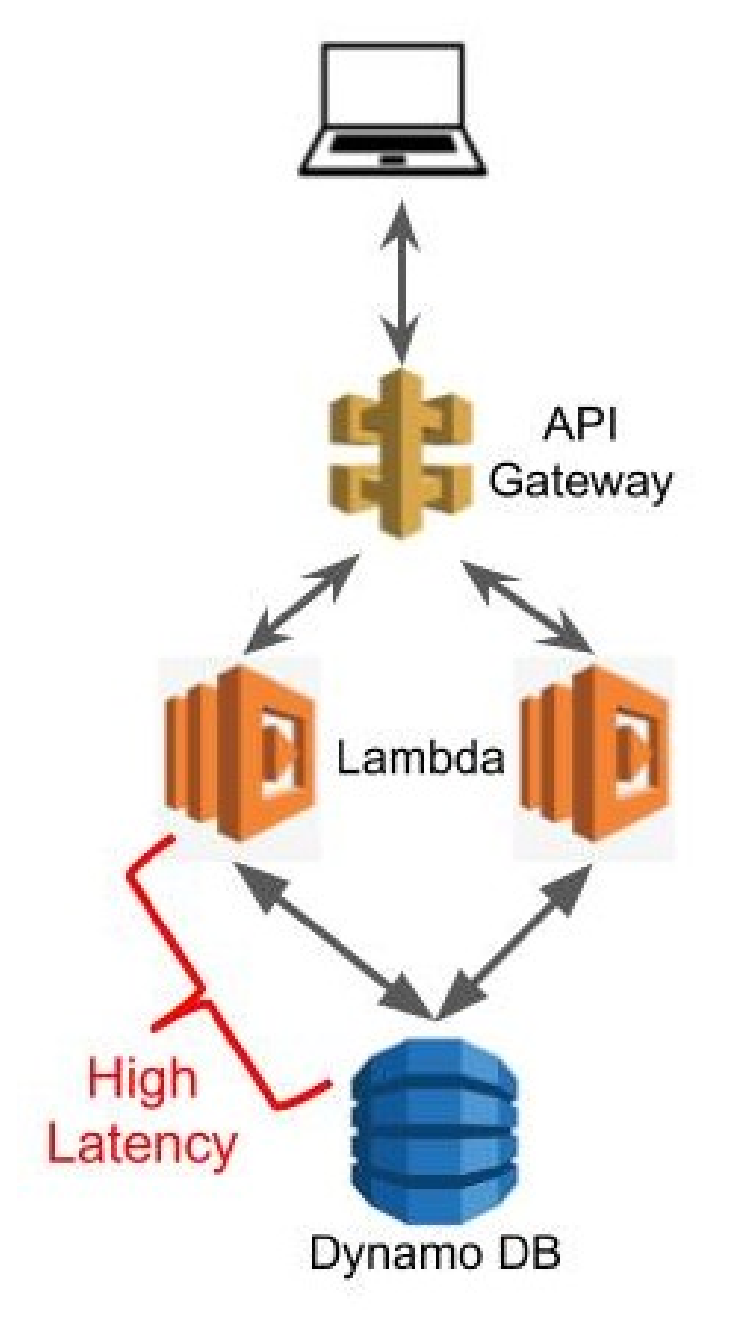
\includegraphics[width=0.5\linewidth, height=0.8\columnwidth]{image/serverless_arch.eps}
%	\caption{Serverless Architecture}\label{fig:serverless_arch}
%\end{figure} 

%\subsection{Some popular serverless usecasess and their archtechture:}
Currently, most of the technology adopters are startups who seek for a possibility to scale painlessly and to lower the entrance barrier. Serverless is also a perfect approach for applications that do not run continuously but rather have quiet periods and peaks of traffic. This concept can be useful for a wide range of applications, from a simple database (DB) application to complex data analytics pipeline applications \cite{Bhattacharjee_USENIX_2019}.
%\begin{enumerate}
%	\item \textbf{Simple DB appliacation:} For any small scale application such as iteractive web site, ERP solutions etc. Serverless is a good candidate to opt as a deployment technology. Figure \ref{fig:simpleDB_serverless} illustrate a simple DB application.
%	
%	\item \textbf{Data analytics pipeline:}
%	\cite{Bhattacharjee_USENIX_2019}.
%\end{enumerate}
% 

%Related work
In the literature, a few recent works have significantly explored serverless computing from different perspectives. In \cite{Akkus_Sand_Usenix_2018}, a new serverless computing system that provides lower latency, better resource efficiency and more elasticity than existing serverless platforms is discussed. To achieve these properties, authores have introduced a model SAND, based on application-level sandboxing and an hierarchical message bus. Here, the design and implementation of SAND, as well as experience in building and deploying serverless applications on it are presented. In \cite{Oakes_USENIX_2018}, the author has analyzed Linux container primitives, identifying scalability bottlenecks related to storage and network isolation where there is a container system optimized for serverless workloads. Based on these findings, they have implemented SOCK, a container system optimized for serverless workloads model. They have identified container initialization and package dependencies as common causes of slow Lambda startup. In \cite{Hong_USENIX_2018}, author has advocated for taking a serverless approach by proposing six serverless design patterns to build security services in the cloud. For each design pattern, they describe the key advantages and present applications and services utilizing the pattern. Using the proposed patterns as building blocks, they have introduced a threat intelligence platform that collects logs from various sources,  alerts malicious activities, and takes actions against such behaviors.

%%\cite{Ishakian_2018}.

Though advantageous in focusing on the user's business logic rather than the platform management, serverless architectures has latency related issues as it is stateless and need to communicate with data source, other serverless functions. In this paper, we analyze this latency of serving requests for different serverless architectures. First, we take the simplest use case of a database application and compare the performance with the traditional VM based approach. Next, we analyze a more complex data pipeline involving multiple functions and observe how it impacts the overall latency of the service. Then, we propose some simple caching strategies to improve the response times. Finally, we discuss their pitfalls.

%Our contributions include:
%(1) Showing database access in AWS lambda function is 80 times more expensive than using traditional VMs.
%(2) Using in memory key value stores like Redis can significantly reduce the latency of database access.
%(3) The lambda containers can cache data for faster access, and it is persisted till a cold start is hit. However there are some challenges as discussed.
%(4) Cascading serverless functions incurs a very big latency penalty.
%(5) Analyze Geo distributed serverless architectures
\section{Latency Analysis}\label{latencyanalysis}
In order to understand the latency of serverless architectures in AWS Lambda services, we considered two practical use cases:
(1) Simple database applicaton
(2) Complex data analytics pipeline. We compare the latency of the serverless system with a traditional cloud VM based setup and also see how this latency is affected as the system scales to more complex architectures.

\begin{figure}[ht]
	\centering
	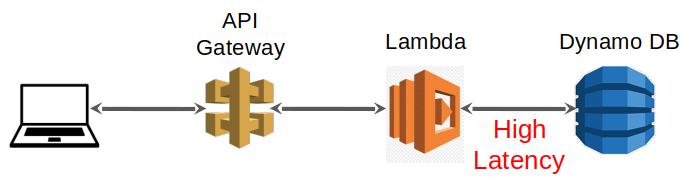
\includegraphics[width=0.7\linewidth]{image/simpleDB_serverless.png}
	\caption{Serverless for simple DB Application}\label{fig:simpleDB_serverless}
\end{figure}


\begin{figure}[ht]
	\centering
	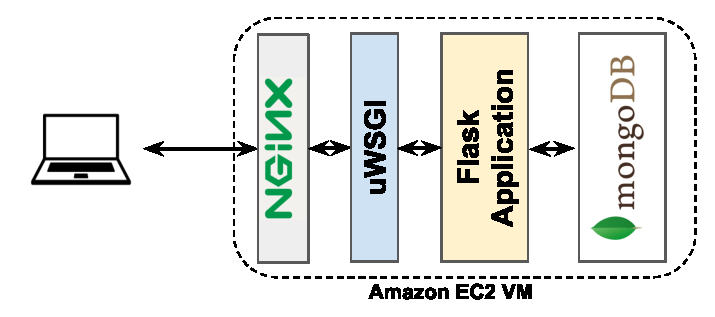
\includegraphics[width=0.7\linewidth]{image/flaskmongo.eps}
	\caption{VM based setup using Flask and MongoDB on AWS EC2}\label{fig:vmbasedsetup}
\end{figure}


\begin{figure}[ht]
	\centering
	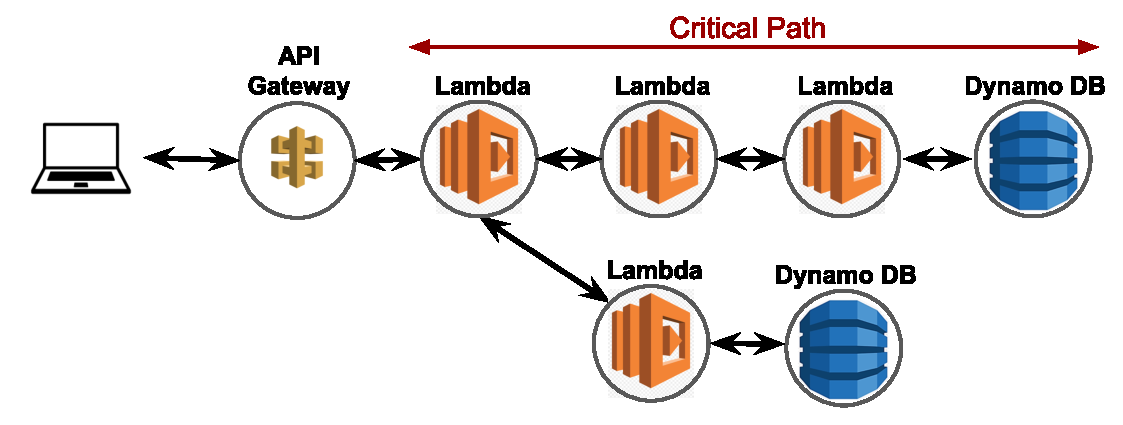
\includegraphics[width=0.8\linewidth]{image/complexserverless.eps}
	\caption{Serverless for Data analytics pipeline Application}\label{fig:DataAnalytics_serverless}
\end{figure}

\subsection{Methodology}
(1) \textbf{Simple database applicaton}: This involves only one Lambda function and one database. As the serverless functions are stateless and unlike VM we cannot save any data on it, we use Amazon's \textit{DynamoDB}\footnote{https://aws.amazon.com/dynamodb/ (Last accessed \today)}, which is a key-value and document database. In order to access the service we connect the Lambda function to an API Gateway through which it can accept HTTP requests. The architecture is depicted in Figure \ref{fig:simpleDB_serverless}. We implemented a simple application in a single lambda function using Node JS to store and retrieve account details of users from the database. In order to compare the performance of this setup relative to the traditional cloud VM based approach, we also implemented a web service with the same functionality in a VM on Amazon EC2\footnote{https://aws.amazon.com/ec2/ (Last accessed \today)} service. For this setup we used Python Flask\footnote{http://flask.palletsprojects.com (Last accessed \today)} web framework along with MongoDB as a database (Figure \ref{fig:vmbasedsetup}). The Flask application is served through Nginx\footnote{http://nginx.org/ (Last accessed \today)} web server and uWSGI\footnote{https://uwsgi-docs.readthedocs.io/en/latest/ (Last accessed \today)} application server. All these components run on the same VM with 1 vCPU and 1 GB of memory. We deployed both the  serverless and server based setups in five data centers in different regions namely, Mumbai, London, California, Canada central and Singapore. In order to make a fair comparison, to eliminate the factor of network quality delay from the end user, we only consider the time taken to process the user's request by the serverless setup and the traditional VM based setup. For serverless setup we use CloudWatch\footnote{https://aws.amazon.com/cloudwatch/ (Last accessed \today)} logs, and for server based setup we use Nginx logs to get the response time of the service.

(2) \textbf{Complex data analytics pipeline}: Here we take into account multiple lambda functions which are common for data analytics pipelines, data mining workflows, and any other complex applications involving multiple steps and processes. Any such workflow can be depicted like a graph, where the vertices are serverless components such as logic units like Lambda functions, databases like DynamoDB, file stores like Amazon S3, cache services such as Redis, etc.. There exists an edge between two such vertices if one component calls the other component and waits for its response. Or in other words, there is an edge between two components if one component depends on another component.
Thus, it is expected that the response time of the service will be equal to the sum of the computation time of the components in the longest path of the graph which is the critical path. However, since the functions and components are managed by the provider, here AWS, we do not have any control of their deployment except ensuring that they are deployed in the same region. As a result, the lambda functions, databases, and other services are deployed in different hosts and must communicate through the network which incurs some delay. This delay between each component ultimately has a severe cascading effect on the overall response time of the application. We analyzed the overall latency with different workflows of varying critical path lengths involving a series of Lambda functions terminating at DynamoDB (Figure \ref{fig:DataAnalytics_serverless}).


\subsection{Observations}

\begin{figure}[h]
	%\begin{minipage}{0.24\textwidth}
	\center
	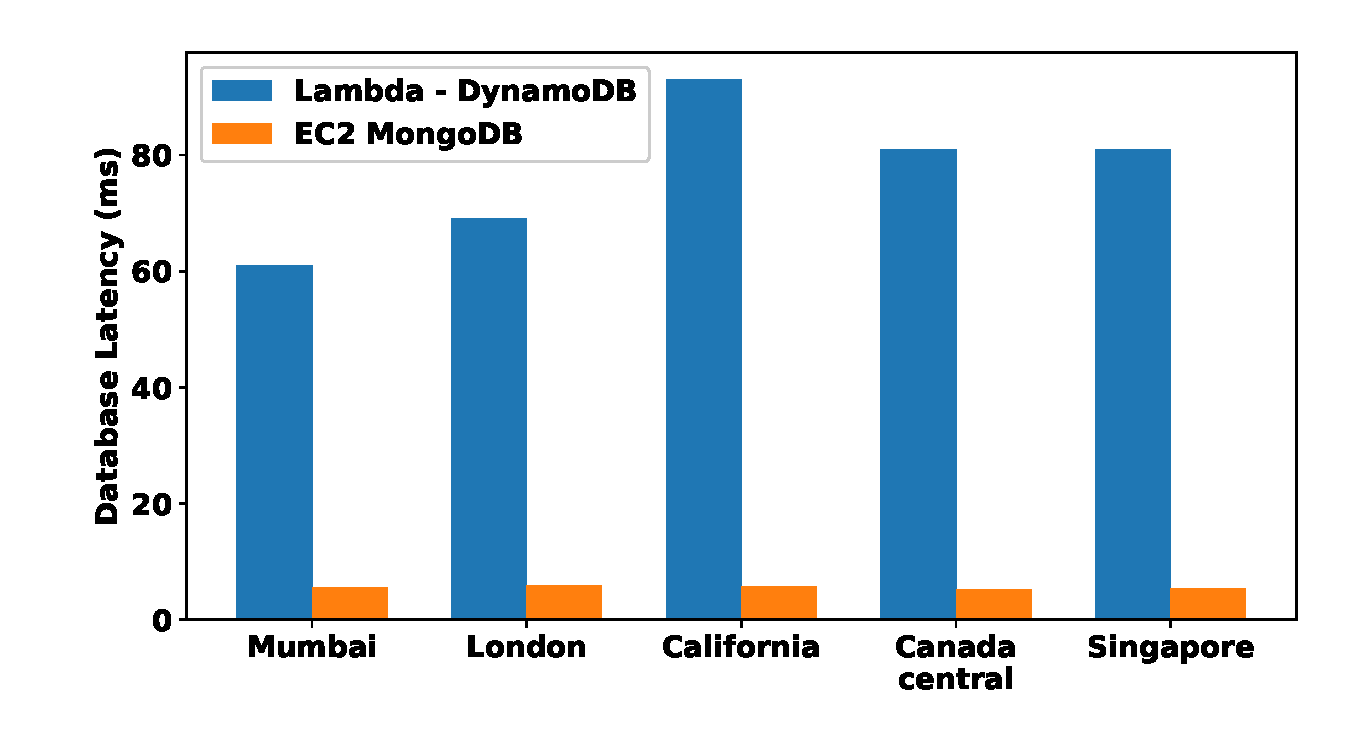
\includegraphics[width=0.9\linewidth]{image/dblatency.eps}
	\caption{DynamoDB $vs.$ MongoDb.}\label{fig:DynamoDBvsMongoDb}
	%\end{minipage}
\end{figure}


\begin{figure}[h]
	%\begin{minipage}{0.24\textwidth}
	\center
	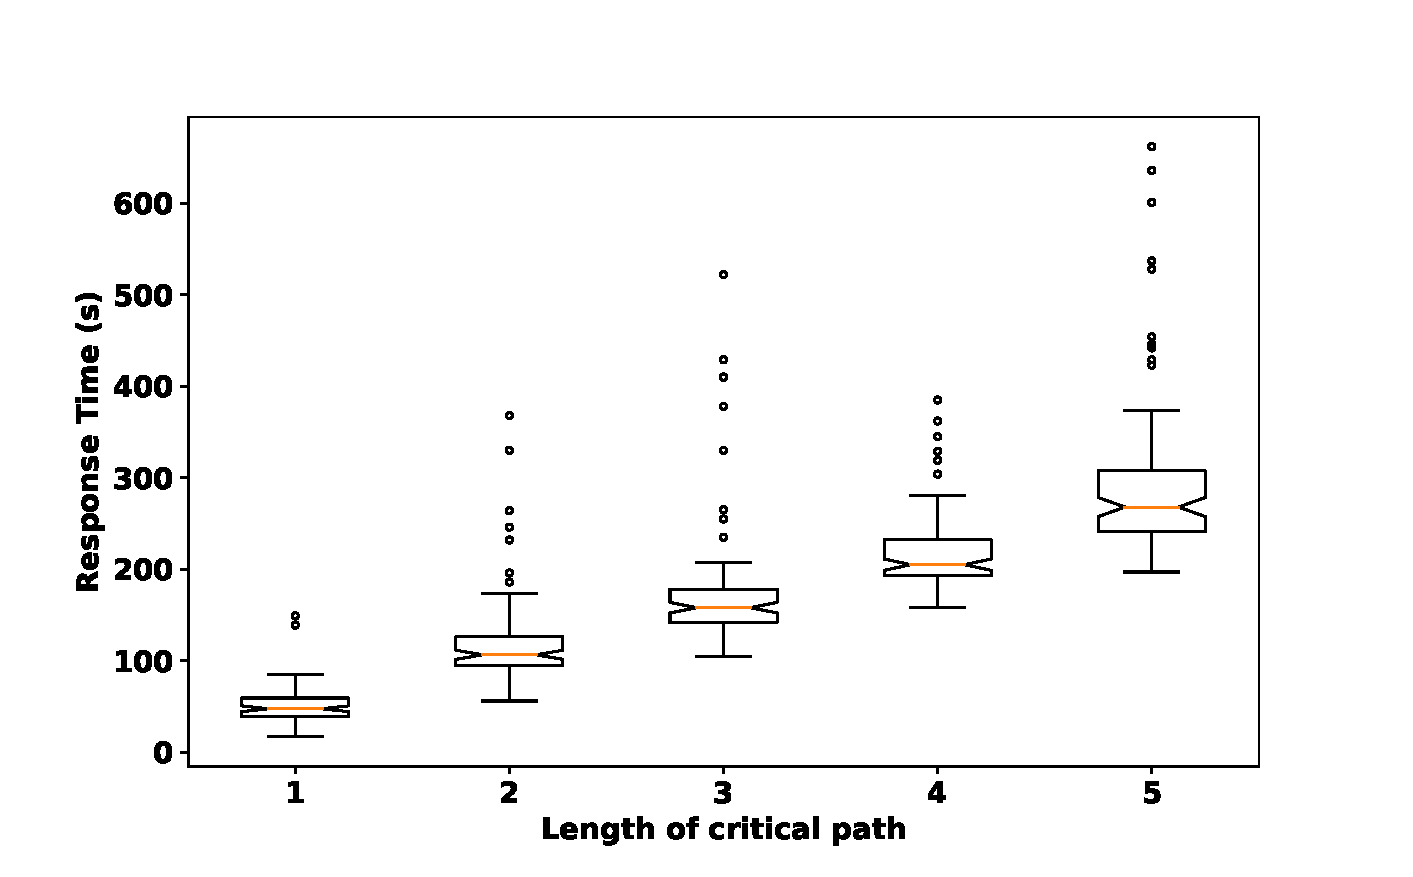
\includegraphics[width=\linewidth]{image/cascadinglatency.eps}
	\caption{serverless Cascading Data.}\label{fig:serverlessCascadingData.png}
	%\end{minipage}
\end{figure}



For the simple database application involving only a single database read or write operation per request, we measure the response time of the system per user request. We deployed both the serverless setup and the VM based setup in five regions. We observed that the  response time for the serverless architecture is significantly higher than the VM based setup. After a careful study we found that the reason of this higher latency is not because of higher processing time by the lambda function but mostly due to the latency of the database access.  In Figure \ref{fig:DynamoDBvsMongoDb}, we compare the mean database access times by the Lambda function and the Flask web application to the DyanamoDB and MongoDB respectively, in five regions. Clearly, in all regions the access time of the database in serverless setup is significantly higher than in case of the VM based setup. The most probable reason behind this is since in serverless the database and the Lambda function are not necessarily hosted on the same physical host, the DynamoDB access involves network latency, in contrast to MongoDB which is hosted in the same VM. Overall, the database access time in serverless architecture is nearly 14 times of that in traditional VM based architecture if the database is hosted in the same VM.

In the second scenario, we compared the latency of the serverless architectures with varying critical path length. The smallest such setup is of length $1$, which includes only one Lambda function and a database just like the first case. For the architecture of length $2$, the longest path involves two Lambda functions and one database at the end. Similarly we deployed such setups of critical path length $3$,$4$ and $5$. Each of the Lambda function has negligible computation and their individual response times are less than $5ms$. This allows us to monitor only the overhead due to the chaining of serverless components through network calls. Figure \ref{fig:serverlessCascadingData.png} shows the box and whisker plot of the distribution of response time for 100 user requests. We can observe that the response time of the system increases steadily with increasing length of the architecture. The mean latency of the system increases by 7.6 times from $50ms$ in case of length 1 to $430ms$ for length 5. Thus, as the serverless architectures grow more and more complex, it incurs more and more latency overhead.


\section{Serverless Caching}\label{caching}
In both the scenarios, the overall latency is a result of the network delay in between the components of the architecture. Often, this network calls can be completely avoided by caching previously computed results. However, unlike in traditional cloud VMs, in Lambda functions there is no provision to install an in-memory cache service such as Memcache, Redis etc.. Each of the requests it receives are treated separately and processed separately. AWS provides separate services such as Redis and Memcache through \textit{Amazon ElastiCache}. But although using it will avoid computational time, since they are not in the same container or host as the other components, they also have the overhead of network calls.
In order to reduce the latency futher by avoiding any network calls, we propose a memory caching technique by leveraging the Lambda container's presistency across multiple consecutive requests in short invervals and Javascript's asynchronous function calls for lazy cache updates.

\begin{figure}[h]
	%\begin{minipage}{0.24\textwidth}
	\center
	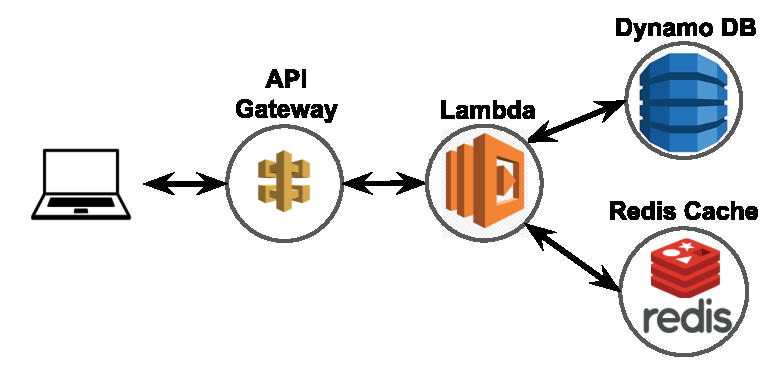
\includegraphics[width=0.8\linewidth]{image/rediscache.eps}
	\caption{Redis as a cache}\label{fig:rediscache}
	%\end{minipage}
\end{figure}


\begin{figure}[h]
	%\begin{minipage}{0.24\textwidth}
	\center
	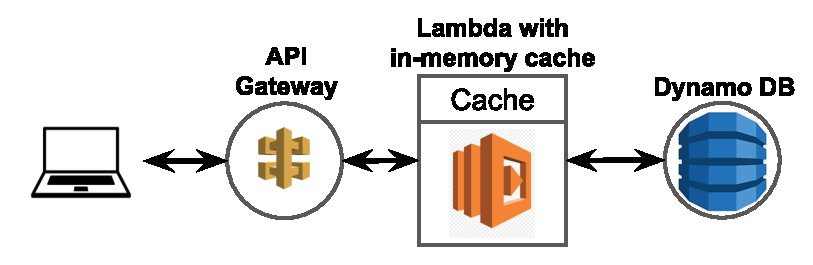
\includegraphics[width=0.8\linewidth]{image/memorycache.eps}
	\caption{In-memory cache}\label{fig:memorycache}
	%\end{minipage}
\end{figure}
\section{Evaluation}\label{eval}
In order to compare the performance with different caching techniques, we setup a simple database application involving Dynamo DB and a Lambda function. Along with that we implement Redis and our proposed memory caching techniques (Figure XX). Figure \ref{fig:RedisVsMemoryVsDynamoDB} shows the response time for different caching techniques.


\begin{figure}[h]
%\begin{minipage}{0.24\textwidth}
\center
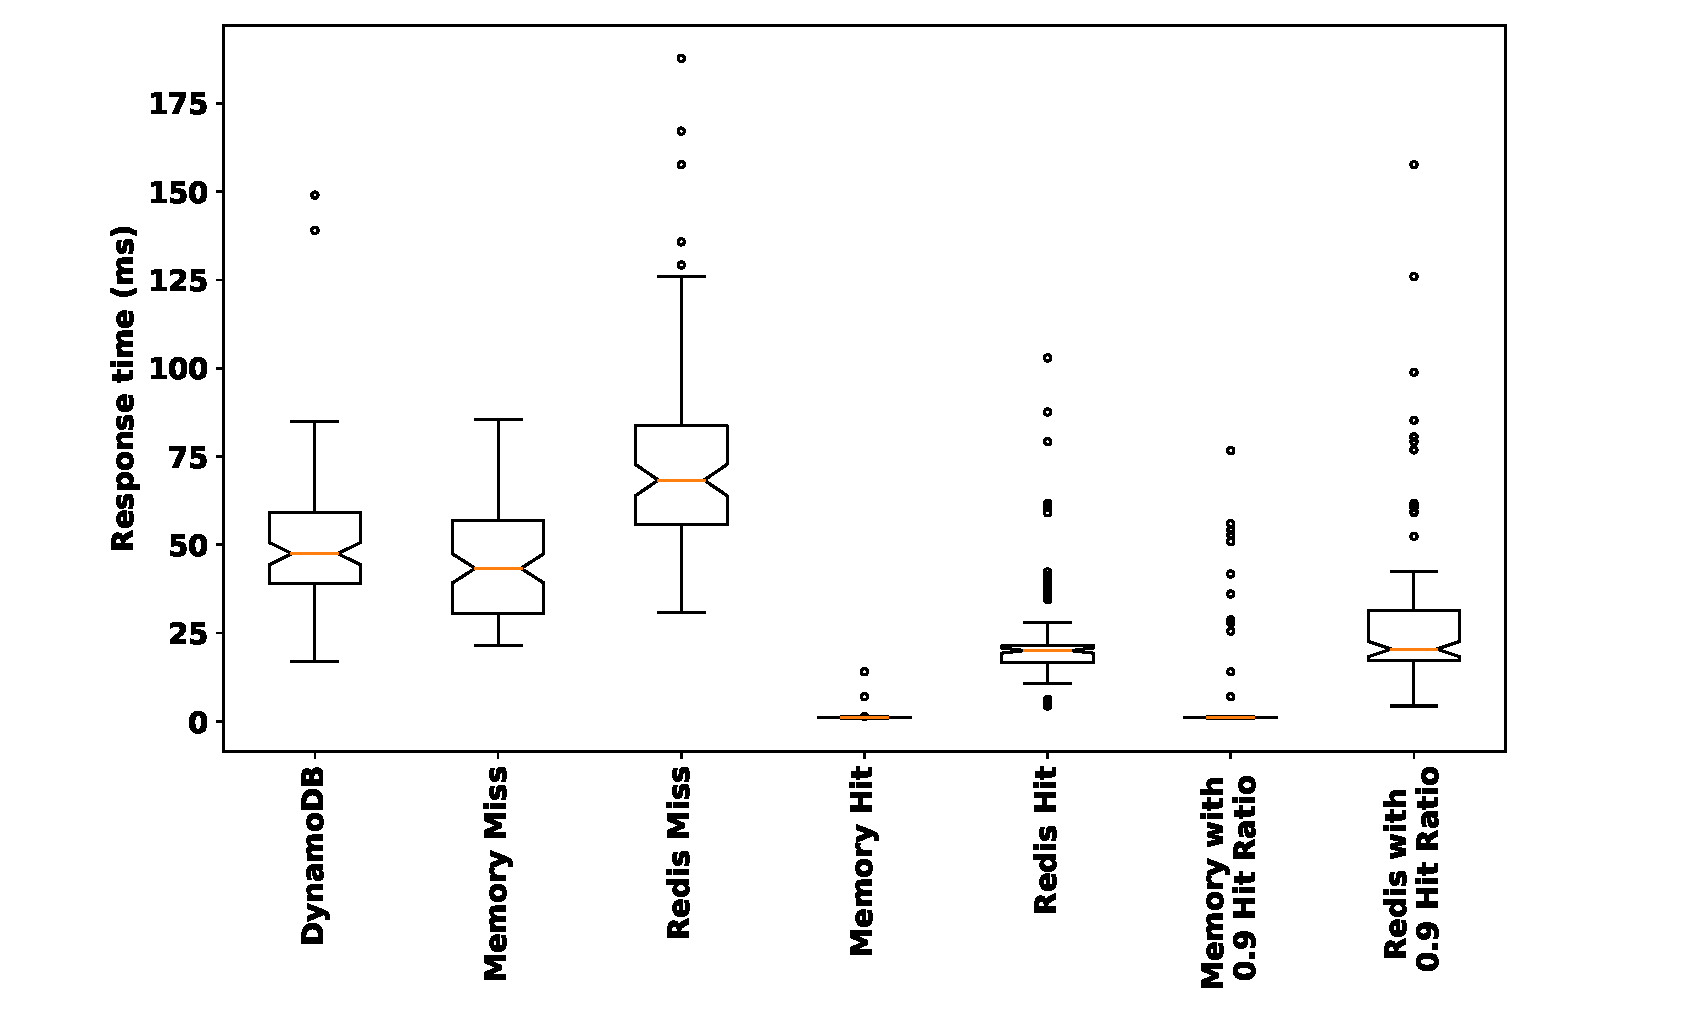
\includegraphics[width=\linewidth]{image/redismemoryresults.eps}
		\caption{Redis $vs.$ Memory $vs.$ DynamoDB.}\label{fig:RedisVsMemoryVsDynamoDB}
%\end{minipage}
\end{figure}

\section{Conclusion}\label{conlsn}
To develope and deploy complex services serveless is a good candidate. Howevere, the latency incured between the user, lambda and DB is a important issue, which may leads to the less QoE for any service. In this work, we analyze different serverless architectures with AWS Lambda services and compare their performance in terms of latency with traditional virtual machine based approach. We then compare some caching strategies which can improve the response times thus improving quality of experience of the end-users.  
For an immidate extenssion of this work we have......

\ifCLASSOPTIONcaptionsoff
  \newpage
\fi

\bibliographystyle{IEEEtran}
\bibliography{biblio}

\end{document}


